\section{PGFplotstable}

The figure data i nthe figure was 

\begin{figure}
    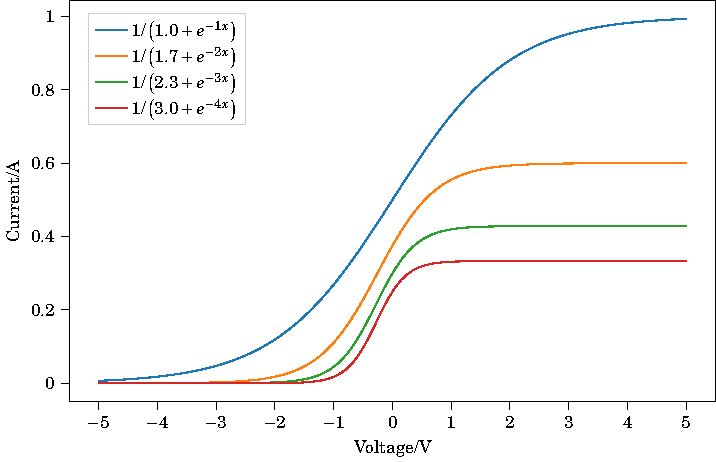
\includegraphics[width=0.5\textwidth]{example_3}
\end{figure}


\begin{table}[htbp] 
    \caption{Generated with PGFplotstable}
    \centering
    \pgfplotstabletypeset[
        col sep=comma,
        every column/.style={fixed zerofill,precision=2},        
        columns/0/.style={
            column name={No}, 
            precision=0},
        columns/alpha/.style={
            column name={$\alpha$}, 
            precision=2},
        columns/beta/.style={
            column name={$\beta$}, 
            precision=1},
        every head row/.style={before row=\toprule,after row=\midrule},	% style the first row
        every last row/.style={after row=\bottomrule},	% style the bottom row
        ]{./tabs/example_3.csv}
\end{table}